% !TeX spellcheck = nl_NL
\begin{savequote}[0.55\linewidth]
	``Optimization before measurement is the root of all evil''
	\qauthor{\textasciitilde D. Knuth}
\end{savequote}

\chapter{Implementatie}
\label{chap:implementatie}

Om een zo eerlijk mogelijke vergelijking te bekomen, zullen we zowel bij de client-side implementatie van Linked Connections als de server-side API (LC2Irail) dezelfde algoritmes toepassen. Gezien de jonge leeftijd van het Linked Connections framework zijn er nog geen algoritmes beschikbaar om deze data te verwerken. We zullen de ontwikkeling van deze algoritmen bespreken, met speciale aandacht voor het routeplanning algoritme vanwege de hogere complexiteit en de uitgebreide mogelijkheden.

\section{Linked Connections specificaties}
\label{sec:lcformaat}
Zoals eerder aangehaald publiceert Linked Connections geen dump van reisinformatie of een volledige routeplanner, maar een lijst van zogenoemde connecties. Een connectie is het kleinste ondeelbaar stuk van een treinrit, en beschrijft het vertrek in een station en de aankomst in het volgende station op de route. Deze connecties worden opgeslagen in een lijst en gesorteerd volgens vertrektijd. Hierna wordt deze lijst gesplitst, om pagina's van gelijke grootte of gelijke tijdsduur te bekomen. Deze fragmenten kunnen gepubliceerd worden via HTTP als \foreign{JSON-LD}\footnote{https://json-ld.org/}, waarbij user-agents kunnen kiezen welke pagina's ze opvragen. Links in de gepubliceerde documenten zorgen ervoor dat user-agents steeds weten welke pagina ze als volgende moeten laden~\citep{linkedconnections18}.

Om bovenstaande methode in de praktijk om te zetten, wordt gebruikgemaakt van de open source LC-Server\footnote{https://github.com/julianrojas87/linked-connections-server/}. Om GTFS om te zetten naar Linked Connections, wordt er achterliggend gebruikgemaakt van de gtfs2lc tool\footnote{https://github.com/linkedconnections/gtfs2lc}.

Deze data zijn publiek toegankelijk via https://graph.irail.be/.

\subsection{Vraag- en antwoordformaat}
Om een pagina met data op te halen, wordt een verzoek gemaakt naar de API, waarbij de vervoersmaatschappij en het gewenste tijdstip in ISO8601 formaat in de URL opgenomen worden. In codefragmenten~\ref{code:2:linkedconnections-response-context} en~\ref{code:2:linkedconnections-response-graph} zien we het resultaat voor de NMBS op 20 maart 2018, 12:30. Het verzoek dat gemaakt werd om de resultaten te bekomen is een HTTP verzoek naar \inlinecode{\url{https://graph.irail.be/sncb/connections?departureTime=2018-03-20T12:30:00.000Z}}.

We overlopen nu de belangrijkste velden in dit antwoord:
\begin{enumerate}
	\item \foreign{@context}: Deze lijst, zichtbaar in codefragment~\ref{code:2:linkedconnections-response-context}, definieert de gebruikte namespaces en velden
	\item \foreign{hydra:next} en  \foreign{hydra:previous}: Links naar de pagina met respectievelijk de volgende en de voorgaande data
	\item \foreign{hydra:search}: Informatie over de huidige pagina
	\item \foreign{@graph}: Deze lijst, zichtbaar in codefragment~\ref{code:2:linkedconnections-response-graph},  bevat de eigenlijke data. Elk vertrek bevat de volgende informatie:
	\begin{enumerate}
			\item \foreign{departureStop}: De URI welke het station van vertrek uniek identificeert.
			\item \foreign{arrivalStop}: De URI welke het station van aankomst uniek identificeert.	\item departureTime, arrivalTime: De geplande tijden, respectievelijk bij vertrek en aankomst.
			\item \foreign{departureDelay}, \foreign{arrivalDelay}: De vertraging, respectievelijk bij vertrek en aankomst.
			\item \foreign{direction}: De richting van dit voertuig, wat vaak ook op de lichtkrant van het voertuig weergegeven wordt.
			\item \foreign{gtfs:trip}: Een URI welk de rit van het voertuig uniek identificeert
			\item \foreign{gtfs:route}: Een URI welk de route van het voertuig uniek identificeert
			\item \foreign{gtfs:pickupType} en \foreign{gtfs:dropOffType}: geeft aan of reizigers al dan niet kunnen op- of afstappen bij respectievelijk vertrek en aankomst
	\end{enumerate}
\end{enumerate}

\begin{listing}[h]
	\begin{minted}[breaklines,tabsize=2]{json}
			{"@context": {
			    "lc": "http://semweb.mmlab.be/ns/linkedconnections#",
			    "hydra": "http://www.w3.org/ns/hydra/core#",
			    "gtfs": "http://vocab.gtfs.org/terms#",
			    "...": "..."
			},
			"@id": "https://graph.irail.be/sncb/connections?departureTime=2018-03-20T12:30:00.000Z",
			"@type": "hydra:PagedCollection",
			"hydra:next": "https://graph.irail.be/sncb/connections?departureTime=2018-03-20T12:40:00.000Z",
			"hydra:previous": "https://graph.irail.be/sncb/connections?departureTime=2018-03-20T12:20:00.000Z",
			"hydra:search": {"...": "..."},
			"...":"..."}
		\end{minted}
	\caption{Voorbeeld Linked Connections formaat: context}
	\label{code:2:linkedconnections-response-context}
\end{listing}
\begin{listing}[h]
	\begin{minted}[breaklines,tabsize=2]{json}
			{"...":"...",
			"@graph": [
				{   "@id": "http://irail.be/connections/8822228/20180320/S11961",
				    "@type": "Connection",
    				"departureStop": "http://irail.be/stations/NMBS/008822228",
    				"arrivalStop": "http://irail.be/stations/NMBS/008822210",
    				"departureTime": "2018-03-20T12:30:00.000Z",
    				"departureDelay": 60,
    				"arrivalTime": "2018-03-20T12:32:00.000Z",
    				"arrivalDelay": 0,
    				"direction": "Anvers-Central",
    				"gtfs:trip": "http://irail.be/vehicle/S11961/20180320",
    				"gtfs:route": "http://irail.be/vehicle/S11961",
    				"gtfs:pickupType": "gtfs:Regular",
    				"gtfs:dropOffType": "gtfs:Regular"
				},
				{"...":"...", }
			]}
	\end{minted}
\caption{Voorbeeld Linked Connections formaat: graph}
\label{code:2:linkedconnections-response-graph}
\end{listing}
 
De volledige specificatie kan teruggevonden worden op de LC website\footnote{https://linkedconnections.org/specification/1-0}.
 
\subsection{Open World Assumption}
Een van de speerpunten van Linked Connections is het gemak waarmee data gecombineerd kunnen worden. Om data van meerdere vervoersmaatschappijen te combineren, hoeft men enkel de Linked Connections voor deze vervoersmaatschappijen te downloaden, en \foreign{merge-sort} toepassen. Wanneer het niet mogelijk is een route tussen twee punten te plannen, is het ook nog steeds mogelijk dat deze route gepland kan worden wanneer data van een extra vervoersmaatschappij toegevoegd wordt. Dit heet de Open World Assumption. Formeel stellen we dat de open world assumption gedefinieerd wordt door de veronderstelling dat de "waarheid" van een statement of hypothese niet afhangt van het al dan niet bekend zijn van deze hypothese door een enkele agent~\citep{Moore15}. Met andere woorden is mogelijk dat wanneer een client een vraag niet kan beantwoorden, het nog steeds mogelijk is dat er een antwoord op deze vraag is wanneer meer data toegevoegd wordt.


\section{Gebruikte systemen doorheen dit onderzoek}
In het kader van dit onderzoek zullen we twee implementaties ontwikkelen. Enerzijds ontwikkelen we een client-side implementatie van Linked Connections, waarbij data opgehaald wordt van de bestaande Linked-Connections-Server. Anderzijds ontwikkelen we ook een RPC API die als referentie zal dienen, LC2Irail. Deze API hanteert dezelfde algoritmes als de lokale implementatie.

\textbf{Linked Connections Server} Deze term doelt op de bestaande NodeJS applicatie welke Linked Connections fragmenten beheert op een server, en deze over HTTP aanbiedt. Beide API implementaties maken gebruik van deze fragmenten. Broncode is beschikbaar op https://github.com/julianrojas87/linked-connections-server/.

\textbf{Linked Connections, LC, lokale implementatie} Deze termen doelen op de implementatie waarbij data van de Linked-Connections-Server opgehaald wordt en op het mobiele toestel verwerkt wordt. Broncode is beschikbaar op https://github.com/Bertware/masterthesis-LC-LC2Irail-android-client.

\textbf{LC2Irail, server implementatie} Deze termen doelen op de implementatie van een RPC API waarbij data in de vorm van Linked Connections fragments van de harde schijf opgehaald wordt, om daarna op de server verwerkt te worden en het antwoord naar de mobiele client te sturen. Broncode is beschikbaar op https://github.com/Bertware/masterthesis-lc2Irail.

Zowel de implementatie op basis van de \foreign{org.json} parser en de implementatie op basis van de \foreign{LoganSquare} parser kunnen gedownload en geïnstalleerd worden door de *.apk bestanden te downloaden op een smartphone met Android 4.4 of hoger. De applicatie is beschikbaar op \url{https://github.com/Bertware/masterthesis-LC-LC2Irail-android-client/releases/tag/RESEARCH40}.

Beide implementaties beschikken elk over dezelfde drie types opzoeking.

\textbf{Liveboards} Deze opzoeking geeft de gebruiker alle vertrekkende of aankomende treinen voor een bepaald station. Er zijn theoretisch gezien oneindig veel resultaten beschikbaar door het beschouwde tijdsinterval steeds uit te breiden.

\textbf{Routes} Deze opzoeking geeft de gebruiker routes van A naar B, waarbij stations A en B door de gebruiker zijn gekozen. Er zijn theoretisch gezien oneindig veel resultaten beschikbaar door het beschouwde tijdsinterval steeds uit te breiden.

\textbf{Voertuigen} Deze opzoeking geeft het volledige traject van een voertuig weer. Het volledig traject wordt als één resultaat beschouwd.

\section{Algoritmes}
\label{sec:algoritmes}
\subsection{Connection Scan Algoritme}
\label{sec:csa}
Veelgebruikte algoritmes voor routeplanning zijn (varianten op) het algoritme van Dijkstra~\citep{Dijkstra59, strasser13,hannemann07,hannemann08} of Bellman-Ford~\citep{Bellmanford58}. Toepassingen die gebruik maken van deze algoritmes vereisen echter het bijhouden van een graaf, en in het geval van Dijkstra ook een \foreign{priority queue}. Naast de impact op prestaties die deze eisen vormen, beperkt een graaf ook de flexibiliteit. De \foreign{Open World Assumption} stelt dat er steeds andere stopplaatsen zijn wiens bestaan we (nog) niet kennen. Het opstellen van een graaf zou vereisen dat we alle gegevens eerst volledig moeten downloaden, terwijl Linked Connections net goed geschikt is voor streaming. 

Het Connection Scan Algoritme (CSA) werd voor het eerst beschreven door Ben Strasser in 2013~\citep{strasser13}. Dit algoritme vereist een lijst met vertrekken gesorteerd op vertrektijd. Hiermee worden alle routes in een tijdsinterval efficiënt berekend~\citep{strasser14,strasser17}. In tegenstelling tot Dijkstra's algoritme is er geen graaf of \foreign{priority queue} nodig. Waar andere algoritmen ofwel enkel op kleine netwerken performant zijn, ofwel niet altijd de best mogelijke route vinden, kan CSA de optimale route in grote netwerken toch efficiënt vinden~\citep{strasser14}.

In de praktijk blijkt de standaard implementatie van CSA snel genoeg voor realtime opzoekingen, ook voor grote spoornetwerken zoals het Duitse net~\citep{strasser14}. Wanneer Linked Connections op grote schaal toegepast wordt, kan ook de performantie van CSA nog verder verbeterd worden door het implementeren van Connection Scan Accelerated~\citep{strasser14,strasser17}. Een andere optie is het toepassen van heuristieken. Deze verbeteren wel de responstijd, maar zorgen er in sommige gevallen voor dat een optimale route niet gevonden wordt~\citep{hannemann07}. Gezien het Belgische spoornetwerk relatief klein is in vergelijking met andere landen, zullen we hier rechtstreeks CSA op toepassen zonder van verdere heuristieken gebruik te maken. 

Wanneer we een routeplanning algoritme willen gebruiken voor een spoornetwerk, is het vooral belangrijk om snel rekening te kunnen houden met vertragingen bij vertrek of aankomst~\citep{strasser14,strasser17}. Als een trein met vertraging zal vertrekken, hoeft enkel de connectie die bij dit vertrek hoort aangepast te worden. Hierna zal CSA weer correcte resultaten geven rekening houdend met de vertraging. Met andere woorden hoeven we dus gewoon de Linked Connections-pagina opnieuw te laden om een nieuwe lijst te verkrijgen met de huidige vertragingen. 

Net zoals Dijkstra en andere algoritmes berekent CSA de snelste route, al is dit duidelijk niet altijd de route die de gebruiker wenst. Zo kan de snelste route nog steeds een station meermaals bezoeken, of kan men van een trein afstappen om later op deze zelfde trein weer op te stappen~\citep{strasser14}. Terwijl intuïtief duidelijk is dat deze routes niet de beste routes zijn, kan de reistijd bij deze trajecten even lang zijn als de snelste route. Het algoritme kan dergelijke routes dus als antwoord kiezen.

Een oplossing hiervoor is om ervoor te zorgen dat de resultaten pareto-optimaal zijn. Een resultaat is pareto-optimaal als het niet gedomineerd wordt door een ander resultaat. Een resultaat $q$ wordt gedomineerd door een ander resultaat $p$ als $p$ voor minstens één criterium een beter waarde heeft, en voor geen enkel criterium een slechtere waarde heeft dan $q$~\citep{hannemann08,strasser17}. Door ook het aantal overstappen te optimaliseren voorkomen we dat van eenzelfde trein wordt afgestapt om later terug op te stappen~\citep{strasser14}. Een oplossing met een overstap te veel heeft immers een criterium met een slechtere waarde, en zal dus nooit pareto-optimaal zijn.

Naast de tijd van aankomst zijn er nog een aantal andere criteria die vaak geoptimaliseerd worden. Na reistijd is het aantal overstappen het tweede populairste criterium, gevolgd door de prijs van de reis~\citep{strasser17}. Optimalisatie van de prijs is echter zeer complex vanwege de complexe tariefplannen bij openbaar vervoer~\citep{muller06}. Dit valt buiten de context van deze masterproef.

De werking en implementatie van CSA worden uitvoerig behandeld in~\citep{strasser17}. %TODO:correcte zin of ook titel schrijven?
De implementatie en evolutie in dit project zal worden uitgelegd aan de hand van code fragmenten in Java. Er wordt hierbij verondersteld dat sectie 4.2 in~\cite{strasser17} gekend is. De code is asynchroon, waarbij na het laden van de eerste Linked Connections-pagina een \foreign{callback} functie opgeroepen wordt om deze pagina te verwerken. Afhankelijk van het resultaat van deze verwerking, wordt er een nieuwe pagina opgevraagd, of wordt het resultaat doorgegeven aan de oproepende code door middel van callbacks. De volledige broncode van de implementatie is online beschikbaar, zowel in  Java\footnote{\url{https://github.com/Bertware/linkedconnections-android-client/blob/master/Hyperrail/src/main/java/be/hyperrail/android/irail/implementation/linkedconnections/RouteResponseListener.java}} als PHP\footnote{\url{https://github.com/hyperrail/lc2irail/blob/master/app/Http/Repositories/ConnectionsRepository.php}}.

Wanneer CSA geïmplementeerd wordt merken we duidelijke verschillen met de voorgestelde routes door de NMBS. Deze verschillen manifesteren zich vooral in de keuze van het station waar er overgestapt moet worden tussen twee treinen, en de keuze van de tussenliggende treinen indien er meer dan één overstap is. Zo is het mogelijk dat er wordt aangeraden om een trein te nemen langs Brussel-Zuid en Brussel-Centraal tot Brussel-Noord, om van daar een andere trein te nemen die op zijn beurt van Brussel-Noord langs Brussel-Centraal naar Brussel-Zuid rijdt. We zullen dit proberen te voorkomen door enkele aanpassingen door te voeren.
Verder zullen we ook nog aanpassingen doorvoeren om eenvoudig het aantal overstappen te beperken, en om op een meer uitgebreide manier aan \foreign{journey-extraction} te doen. Aangezien CSA de connecties volgens dalende vertrektijd overloopt, moeten we op voorhand weten waar te beginnen. Dit kunnen we niet zomaar weten, en wegens de beperkte tijd is het tijdens deze masterproef niet mogelijk hier een apart algoritme voor te implementeren. Wanneer een gebruiker een vertrekuur kiest, zullen we steeds 4 of 6 uur verder in de verzameling connecties beginnen. Een alternatief zou zijn om het \foreign{Earliest Arrival Time} op te lossen alvorens CSA toe te passen, zoals besproken in sectie~\ref{sec:futurework}.

\begin{listing}[htb]
	\begin{minted}[breaklines,tabsize=2]{java}
	class TrainProfile {
		/**
		* The arrival time at the final destination
		*/
		DateTime arrivalTime;
		
		/**
		* The number of transfers until the destination when hopping on to this train
		*/
		int transfers;
		
		/**
		* The arrival connection for the next transfer or arrival
		*/
		LinkedConnection arrivalConnection;
	}
	
	\end{minted}
	\caption[CSA: Gegevensstructuur voor trips]{In tegenstelling tot~\cite{strasser17} wordt niet enkel de aankomsttijd, maar ook de afstaphalte en het aantal overstappen bijgehouden per trip.}
	\label{code:2:trips}
\end{listing}

Allereerst dienen we twee wijzigingen door te voeren aan de gegevensstructuren. De arrays S en T, waarin respectievelijk zogeheten stopprofielen en aankomsttijden bijgehouden werden, zijn vervangen door een Map, waardoor we onbeperkt nieuwe stations en trips kunnen toevoegen, en deze kunnen opvragen op basis van hun URI. Dit maakt het algoritme geschikt om te werken rekening houdend met de open world assumption.  %TODO: citation needed, explanation needed
In de datastructuur voor een voertuig (fragment~\ref{code:2:trips}) houden we niet enkel bij wanneer we zouden aankomen, maar ook met hoeveel overstappen (beginnend na het opstappen op deze trein) we zouden aankomen, en waar we moeten afstappen van deze trein. Dit laatste is essentieel om niet enkel de aankomsttijd, maar ook de exacte route met alle overstappen te kunnen weergeven. 

\begin{listing}[htb]
\begin{minted}[breaklines,tabsize=2]{java}
  class StationStopProfile {
	/**
	* The departure time in this stop
	*/
	DateTime departureTime;
	
	/**
	* The arrival time at the final destination
	*/
	DateTime arrivalTime;
	
	/**
	* The departure connection in this stop
	*/
	LinkedConnection departureConnection;
	
	/**
	* The arrival connection for the next transfer or arrival
	*/
	LinkedConnection arrivalConnection;
	
	/**
	* The number of transfers between standing in this station and the destination
	*/
	int transfers;
}
	\end{minted}
		\caption[CSA: Gegevensstructuur voor stopprofielen]{In tegenstelling tot~\cite{strasser17} wordt niet enkel de vertrek- en aankomsttijd, maar ook het aantal overstappen en de afstaphalte van de volgende trein bijgehouden.}
	\label{code:2:stations}
\end{listing}


Ook de paren van vertrek- en aankomsttijd per station, zogenoemde profielen, worden vervangen door een meer uitgebreide gegevensstructuur, zichtbaar in fragment~\ref{code:2:stations}. Naast de vertrek- en aankomsttijd houden we nu ook de connectie bij waarmee we vertrekken in dit station op dit tijdstip, en de connectie waarmee we aankomen in het volgend station waar we moeten over- of afstappen. Ook het aantal overstappen, beginnend met tellen na het opstappen in dit station, wordt bijgehouden.

\begin{listing}[htb]
\begin{minted}[breaklines,tabsize=2]{java}
	if (data.connections.length == 0) {
		mLinkedConnectionsProvider.getLinkedConnectionByUrl(data.previous, this, this, null);
		return;
	}
	
	boolean hasPassedDepartureLimit = false;
	for (int i = data.connections.length - 1; i >= 0; i--) {
		LinkedConnection connection = data.connections[i];
		
		if (connection.departureTime.isAfter(mArrivalLimit)) {
			continue;
		}
		if (connection.departureTime.isBefore(mDepartureLimit)) {
			hasPassedDepartureLimit = true;
			continue;
		}
		
		...
	}
	\end{minted}
			\caption[CSA: Overlopen van connecties]{Connecties worden overlopen volgens dalende vertrektijd. Er worden beperkingen gesteld op vertrek- en aankomsttijd.}
	\label{code:2:csaloop}
\end{listing}

Wanneer we de ingeladen connecties willen verwerken, filteren we alle connecties uit de pagina die ofwel te vroeg, ofwel te laat vallen. Zoals te zien in fragment~\ref{code:2:csaloop} stellen we een \foreign{flag} in wanneer we voorbij de vroegst toegelaten vertrekdatum zijn. In dit geval zullen we na het overlopen van deze lijst geen nieuwe lijsten meer ophalen. 

\begin{listing}[htb]
	\begin{minted}[breaklines,tabsize=2]{java}
	 	if (Objects.equals(connection.arrivalStationUri, mRoutesRequest.getDestination().getSemanticId())) {
			T1_walkingArrivalTime = connection.arrivalTime;
			T1_transfers = 0;
		} else {
			T1_walkingArrivalTime = infinite;
			T1_transfers = 999;
		}

		// Determine T2, the first possible time of arrival when remaining seated
		if (T.containsKey(connection.trip)) {
			T2_stayOnTripArrivalTime = T.get(connection.trip).arrivalTime;
			T2_transfers = T.get(connection.trip).transfers;
		} else {
			T2_stayOnTripArrivalTime = infinite;
			T2_transfers = 999;
		}	
		\end{minted}
					\caption[CSA: Bepalen van aankomsttijden]{Het aantal overstappen wordt bepaald bij het bepalen van minimale aankomsttijden}
		\label{code:2:csaT1T2}
\end{listing}

Het bepalen van de aankomsttijd bij wandelen, T1, en de aankomsttijd bij het gezeten blijven in de trein, T2, loopt vrijwel gelijk aan de implementatie uit~\cite{strasser17}. Wandelen van een station naar het eindstation wordt niet ondersteund in onze implementatie. Dit implementeren is relatief eenvoudig door het gebruiken van inter-stop foothpaths~\citep{strasser17,hannemann08}, maar deze data is op dit moment niet beschikbaar, en het verzamelen, opschonen en valideren van deze data valt buiten de context van deze masterproef. In fragment~\ref{code:2:csaT1T2} zien we hoe het aantal overstappen wordt bepaald. In het geval dat er geen aankomst mogelijk is (binnen de beperkte tijd) stellen we zowel de aankomsttijd als het aantal overstappen in op een onrealistisch hoog getal. Dit vereenvoudigt de code aanzienlijk, aangezien er geen rekening gehouden hoeft te worden met het mogelijk leeg zijn van variabelen.

\begin{listing}[htb]
	\begin{minted}[breaklines,tabsize=2]{java}
		if (S.containsKey(connection.arrivalStationUri)) {
			int position = S.get(connection.getArrivalStationUri()).size() - 1;
			StationStopProfile stopProfile = S.get(connection.getArrivalStationUri()).get(position);
			
			while ((stopProfile.departureTime.getMillis() - 300 * 1000 <= connection.getArrivalTime().getMillis() ||
			stopProfile.transfers >= maxTransfers) && position > 0) {
				position--;
				stopProfile = S.get(connection.getArrivalStationUri()).get(position);
			}
			if (stopProfile.departureTime.getMillis() - 300 * 1000 > connection.getArrivalTime().getMillis() && stopProfile.transfers <= maxTransfers) {
				T3_transferArrivalTime = new DateTime(stopProfile.arrivalTime.getMillis() + 240 * 1000);
				T3_transfers = stopProfile.transfers + 1;
			} else {
				T3_transferArrivalTime = infinite;
				T3_transfers = 999;
			}
		} else {
			T3_transferArrivalTime = infinite;
			T3_transfers = 999;
		}
		\end{minted}
		\caption[CSA: Bepalen van aankomsttijden]{Bij een eventuele overstap worden ook extra factoren in rekeningen gebracht.}
		\label{code:2:csaT3}
\end{listing}

Bij de bepaling van T3, terug te vinden in fragment~\ref{code:2:csaT3}, maken we de eerste grote afwijking van het oorspronkelijk algoritme. Om te bepalen of een overstap mogelijk is, moeten er reeds profielen voor dit station bekend zijn. Indien dit het geval is, gaan we op zoek naar het profiel waarbij er genoeg tijd is om over te stappen, maar waarbij het aantal overstappen het maximum aantal niet overschrijdt. 
De intra-footpaths~\citep{strasser17,hannemann08}, nodig voor het bepalen van de tijd die reiziger nodig heeft om over te stappen in een station, worden ingesteld op een standaardwaarde die eventueel door de gebruiker gewijzigd kan worden. Dit is nodig aangezien tijdens de ontwikkeling nog geen officiële waarden gepubliceerd waren\footnote{Sinds april is deze data beschikbaar via iRail: \url{https://github.com/iRail/stations/pull/127}}. 
Wanneer we een overstap vinden die aan deze voorwaarden voldoet, verhogen we het aantal overstappen ook met één. Deze aanpak is eenvoudiger dan de array-gebaseerde aanpak omschreven in~\cite{strasser17}. Het voordeel van deze aanpak is dat automatisch alle snelste opties worden bijgehouden, zolang hun aantal overstappen onder het maximum blijft. 

% TODO title of citation?
In plaats van de door~\cite{strasser17} voorgestelde verhoging van de aankomsttijd met één, om zo routes met een gelijke aankomsttijd maar minder overstappen voorkeur te geven, verhogen we hier de aankomsttijd met een vooraf gedefinieerd aantal seconden. Dit aantal geeft aan hoeveel seconden we langer op een trein wensen te zitten, in plaats van over te stappen. Door dit in te stellen op 240, wordt aangegeven dat een route die er tot 4 minuten langer over doet, met een overstap minder, toch de voorkeur krijgt over de snellere route met meer overstappen. Dit is een eerste veld dat eventueel door gebruikers ingesteld zou kunnen worden om de routes te personaliseren.

Bij het bepalen van de vroegste aankomsttijd (fragment~\ref{code:2:csaT3}), wordt nu ook het aantal overstappen dat bij deze aankomsttijd hoort bepaald, en de connectie waar van de trein afgestapt wordt. Wanneer de aankomsttijd met overstap gelijk is aan de aankomsttijd wanneer de reiziger hier blijft zitten, kiezen we voor de aankomsttijd met overstap. Dit kan contra-intuïtief lijken, maar we moeten hierbij onthouden dat bij aankomsttijd T3 reeds een constante `straftijd` is opgeteld (in dit geval 240 seconden). Hierdoor zullen deze aankomsttijden enkel gelijk zijn indien T2 even veel overstappen bevat. In dat geval verkiezen we om `nu` over te stappen, waarbij `nu` vroeger ligt dan T2: we overlopen alle vertrekken immers van laatst naar vroegst.

\begin{listing}[htb]
\begin{minted}[breaklines,tabsize=2]{java}
if (T3_transferArrivalTime.getMillis() <= T2_stayOnTripArrivalTime.getMillis()) {
	Tmin = T3_transferArrivalTime;
	exitTrainConnection = connection;
	numberOfTransfers = T3_transfers;
} else {
	Tmin = T2_stayOnTripArrivalTime;
	if (T2_stayOnTripArrivalTime.isBefore(infinite)) {
		exitTrainConnection = T.get(connection.trip).arrivalConnection;
	} else {
		exitTrainConnection = null;
	}
	numberOfTransfers = T2_transfers;
}

// For equal times, we prefer just arriving.
if (T1_walkingArrivalTime.getMillis() <= Tmin.getMillis()) {
	Tmin = T1_walkingArrivalTime;
	exitTrainConnection = connection;
	numberOfTransfers = T1_transfers;
}

if (Tmin.isEqual(infinite)) {
	continue;
}
		\end{minted}
		\caption[CSA: Bepalen van vroegste aankomsttijd]{Bepalen van de vroegste aankomsttijd}
		\label{code:2:csaMin}
\end{listing}

Door de extra toevoegingen voor journey extraction en het optimaliseren van de routes, is het bijwerken van de gegevenstructuren aanzienlijk ingewikkelder vergeleken met de originele implementatie. Voor voertuigen houden we niet langer enkel de aankomsttijd, maar ook de afstaphalte bij. Hierbij verkiezen we de halte waarlangs we zo snel mogelijk aankomen, maar bij gelijke aankomsttijd wensen we een zo lang mogelijke periode voor de overstap. Wanneer de aankomsttijd gelijk is, onderzoeken we of de nieuwe afstaphalte (de connectie die op dit moment onderzocht wordt) meer tijd voor een overstap geeft. Indien dit het geval is, werken we de afstaphalte bij. Het bijwerken van een bestaande trip is zichtbaar in fragment~\ref{code:2:csaT}.

\begin{listing}[h]
	\begin{minted}[breaklines,tabsize=2]{java}
        if (Tmin.isEqual(T.get(connection.getTrip()).arrivalTime)
			&& !T.get(connection.getTrip()).arrivalConnection.getArrivalStationUri().equals(mRoutesRequest.getDestination().getUri())
			&& T3_transferArrivalTime.isEqual(T2_stayOnTripArrivalTime)
			&& S.containsKey(T.get(connection.getTrip()).arrivalConnection.getArrivalStationUri())
			&& S.containsKey(connection.getArrivalStationUri())
		) {
			LinkedConnection currentTrainExit = T.get(connection.getTrip()).arrivalConnection;
	
			StationStopProfile stationStopProfile = new StationStopProfile();
			stationStopProfile.departureTime = connection.getDepartureTime();
			stationStopProfile.departureConnection = connection;
		
			stationStopProfile.arrivalTime = Tmin;
			stationStopProfile.arrivalConnection = currentTrainExit;
			
			Duration currentTransfer = new Duration(currentTrainExit.getArrivalTime(), getFirstReachableConnection(stationStopProfile).departureTime);
			
			// New situation
			stationStopProfile.arrivalTime = Tmin;
			stationStopProfile.arrivalConnection = exitTrainConnection;
			Duration newTransfer = new Duration(exitTrainConnection.getArrivalTime(), getFirstReachableConnection(stationStopProfile).departureTime);
			
			// If the new situation is better
			if (newTransfer.isLongerThan(currentTransfer)) {
				TrainProfile trainProfile = new TrainProfile();
				trainProfile.arrivalTime = Tmin;
				trainProfile.arrivalConnection = exitTrainConnection;
				trainProfile.transfers = numberOfTransfers;
				
				T.put(connection.getTrip(), trainProfile);
			}
		}
			
		if (Tmin.isBefore(T.get(connection.getTrip()).arrivalTime)) {
			TrainProfile trainProfile = new TrainProfile();
			trainProfile.arrivalTime = Tmin;
			trainProfile.arrivalConnection = exitTrainConnection;
			trainProfile.transfers = numberOfTransfers;
			
			T.put(connection.getTrip(), trainProfile);
		}
	\end{minted}
	\caption[CSA: Bijwerken T]{Bijwerken van de trips gegevensstructuur.}
	\label{code:2:csaT}
\end{listing}

\begin{listing}[h]
	\begin{minted}[breaklines,tabsize=2]{java}
		StationStopProfile newProfile = new StationStopProfile();
		newProfile.departureTime = connection.getDepartureTime();
		newProfile.arrivalTime = Tmin;
		newProfile.departureConnection = connection;
		newProfile.arrivalConnection = T.get(connection.getTrip()).arrivalConnection;
		newProfile.transfers = numberOfTransfers;
		if (S.containsKey(connection.getDepartureStationUri())) {
			int numberOfPairs = S.get(connection.getDepartureStationUri()).size();
			StationStopProfile existingProfile = S.get(connection.getDepartureStationUri()).get(numberOfPairs - 1);
		
			if (newProfile.arrivalTime.isBefore(existingProfile.arrivalTime)) {
				if (newProfile.departureTime.isEqual(existingProfile.departureTime)) {
					S.get(connection.getDepartureStationUri()).remove(numberOfPairs - 1);
					S.get(connection.getDepartureStationUri()).add(numberOfPairs - 1, newProfile);
				} else {
					S.get(connection.getDepartureStationUri()).add(newProfile);
				}
			}
		} else {
			S.put(connection.getDepartureStationUri(), new ArrayList<StationStopProfile>());
			S.get(connection.getDepartureStationUri()).add(newProfile);
		}
	\end{minted}
	\caption[CSA: Bijwerken S]{Bijwerken van de stops gegevensstructuur.}
	\label{code:2:csaS}
\end{listing}

Het bijwerken van de stopprofielen, zichtbaar in fragment~\ref{code:2:csaS}, is lichtjes aangepast om de efficiëntie te verhogen. De vroegste vertrekken worden nu achteraan toegevoegd. Door deze aanpassing, en het gegeven dat de vertrektijd van de huidige connectie altijd\footnote{We overlopen de lijst immers volgens niet-stijgende vertrektijd} gelijk of kleiner dan de vertrektijd van alle vorige connecties is, hoeven we nu enkel het laatste profiel in de lijst te evalueren.

Als de vertrektijd kleiner of gelijk is, moet de aankomsttijd kleiner zijn. we controleren dus enkel of de aankomsttijd kleiner is, en zo ja, of de vertrektijd kleiner of gelijk is. Afhankelijk van deze laatste controle voegen we een nieuw item toe aan de lijst, of vervangen we het laatste. Aangezien we telkens enkel toevoegen wanneer de aankomsttijd vroeger ligt, zal deze lijst altijd gesorteerd zijn volgens dalende aankomsttijd. Hiermee is bewezen dat deze optimalisatie correct is, en een beter alternatief voor het overlopen van de volledige lijst.

\begin{listing}[h]
	\begin{minted}[breaklines,tabsize=2]{java}
		// Results? Return data
		Route[] routes = new Route[S.get(mRoutesRequest.getOrigin().getSemanticId()).size()];
		
		int i = 0;
		for (StationQuintuple quint : S.get(mRoutesRequest.getOrigin().getSemanticId())
		) {
			// it will iterate over all legs
			StationQuintuple it = quint;
			List<RouteLeg> legs = new ArrayList<>();
			
			while (!Objects.equals(it.arrivalConnection.arrivalStationUri, mRoutesRequest.getDestination().getSemanticId())) {
				// use it.departureConnection and it.arrivalConnection to construct legs of this journey
				legs.add(...);
				it = getFirstReachableConnection(it);
			}
			
			routes[i++] = new Route(legs);
		}
	\end{minted}
	\caption[CSA: Journey extraction]{Journey Extraction door middel van post-processing}
	\label{code:2:csaJourneyExtraction}
\end{listing}

De lijst met volledige routes reconstrueren (fragment~\ref{code:2:csaJourneyExtraction}) is relatief eenvoudig. Voor elk profiel horend bij de locatie van waar de reiziger vertrekt, volgen we de vertrek- en aankomstconnecties. Om bij elke tussenstop de juiste connectie te vinden waarmee de reis verder zal gezet worden, vergelijken we de aankomsttijd uit het stopprofiel waaruit we vertrokken, met de aankomsttijden uit de stopprofielen van de tussenstop (fragment~\ref{code:2:csaJourneyExtractionReachable}). Wanneer deze gelijk zijn, hebben we het volgende deel van de reis gevonden. Hierbij is het belangrijk dat de aankomsttijd ook ´straftijd´ voor eventuele overstappen bevat. Deze wordt dan ook enkel intern gebruikt - zodra aan journey extraction gedaan wordt en informatie voor de gebruiker verzameld wordt, gebruiken we de vertrek- en aankomsttijden die omschreven worden in connecties.

\begin{listing}[h]
	\begin{minted}[breaklines,tabsize=2]{java}
		private StationQuintuple getFirstReachableConnection(StationQuintuple arrivalquint) {
			List<StationQuintuple> it_options = S.get(arrivalquint.arrivalConnection.arrivalStationUri);
			int i = it_options.size() - 1;
				while (i >= 0 && it_options.get(i).arrivalTime.getMillis() != arrivalquint.arrivalTime.getMillis() - 240 * 1000) {
				i--;
			}
			return it_options.get(i);
		}
	\end{minted}
	\caption[CSA: Journey extraction bij tussenstops]{Vinden van volgende vertrek bij tussenstop}
	\label{code:2:csaJourneyExtractionReachable}
\end{listing}

\subsection{Vertrekken en aankomsten per station}
In tegenstelling tot routes, kunnen we om de zogenoemde \foreign{liveboards} te berekenen een eenvoudig algoritme gebruiken. We overlopen alle pagina's, en houden enkel de stops bij die betrekking hebben op het gezochte station. Hiervoor gebruiken we twee lijsten voor respectievelijk de vertrekkende en aankomende connecties. We blijven pagina's overlopen tot de stopvoorwaarde is bereikt. Deze verschilt afhankelijk van de locatie waar we het algoritme implementeren:
\begin{itemize}
	\item Op een webserver blijven we extra pagina's van de schijf laden tot het gewenst aantal resultaten is bereikt, of het gewenste tijdsinterval overlopen is.
	\item Bij een lokale implementatie stoppen we zodra we de pagina hebben afgewerkt waarin de eerste stop beschreven wordt. We maken gebruik van incrementele resultaten, waarbij telkens zo snel mogelijk een klein resultaat wordt berekend. Hierdoor krijgt de gebruiker (in theorie) sneller resultaten te zien.
\end{itemize}

Wanneer de stopvoorwaarde is bereikt, splitsen we de lijsten in drie soorten stops:
\begin{itemize}
	\item Vertrekhalte:  dit zijn de stops van voertuigen die deze stopplaats als begin van hun traject hebben en dus geen informatie over een aankomst bevatten
	\item Eindhalte: dit zijn de stops van voertuigen die deze stopplaats als laatste op hun traject hebben en dus niet meer vertrekken
	\item Stops: dit zijn de stops van voertuigen die een tussenstop maken
\end{itemize}

Om te bepalen tot welke categorie een connectie behoort, dienen we voor elke aankomende connectie in het station te bepalen of er een vertrekkende connectie mee overeenkomt. Komt er een vertrekkende connectie mee overeen, is er sprake van een tussenstop. Komt er geen vertrek mee overeen, is dit een eindhalte. De connecties die vertrekken vanuit het station, en waarmee geen aankomst overeenkomt, zijn dan de vertrekhaltes. 

Bij de implementatie hiervan zorgen we ervoor dat we voor elk vertrek alle aankomsten volgens dalende aankomsttijd overlopen: we verwachten in de meeste gevallen een tussenstop (en dus geen vertrek), en in het geval van een tussenstop zal de aankomst slechts enkele minuten eerder zijn. Door de aankomsten volgens dalende aankomsttijd te overlopen zullen we dus sneller de bijhorende aankomende connectie ontdekken, indien deze bestaat.

Het is duidelijk dat dit algoritme slechts éénmaal de lijst met connecties overloopt. Hieruit volgt dat de efficiëntie $O(n)$ is, met $n$ het aantal overlopen connecties. Gezien we alle connecties voor een bepaald tijdsinterval overlopen, is $n$ evenredig met de drukte van het vervoersnetwerk.

\subsection{Route van een voertuig}

Ook de route van een voertuig afleiden uit Linked Connections data is eenvoudig. Zowel de stops van een trein, als de connecties, zijn chronologisch geordend. We overlopen dus alle connecties, waarbij we telkens de laatst gebruikte connectie $p$ en de huidige connectie $c$ in variabelen bijhouden. 
\begin{itemize}
	\item Wanneer we de eerste connectie ontdekken die betrekking heeft op deze trein, is dit de vertrekhalte. We verwerken deze data en voegen dit toe aan de lijst met stops. We kopiëren $c$ naar $p$.
	\item Wanneer $p$ een connectie bevat, en $c$ de hierop volgende connectie bevat, beschikken we over alle informatie om de tussenstop tussen $p$ en $c$ toe te voegen aan de lijst met stops.
	\item Wanneer alle connecties overlopen zijn, was $c$ de laatste connectie van dit trein. Deze connectie duidt dus de eindhalte aan. We voegen deze toe aan de lijst met stops, en geven een antwoord terug aan de oproepende code.
\end{itemize}

Het bepalen van de route van een trein legt een eerste mogelijk pijnpunt van de Linked Connections-specificaties bloot: hiervoor moeten alle connecties voor een volledige dag opgehaald worden. Er is immers geen enkele manier om te bepalen wanneer een trein vertrekt, of wat de eindhalte is. Hierdoor is er een relatief lange laadtijd om alle fragmenten op te halen, wat enigszins beperkt kan worden door deze asynchroon te laden. Het effect hiervan op de gebruikerservaring zullen we later onderzoeken. 

Het is duidelijk dat dit algoritme slechts éénmaal de lijst met connecties overloopt. Hieruit volgt dat de efficiëntie $O(n)$ is, met $n$ het aantal overlopen connecties. Gezien we net zoals bij liveboards alle connecties voor een bepaald tijdsinterval overlopen, is $n$ ook hier evenredig met de drukte van het vervoersnetwerk.

\section {Implementatie in HyperRail}
De in sectie~\ref{sec:algoritmes} besproken algoritmes zijn zowel server-side als client-side in de HyperRail applicatie geïmplementeerd. Door het gebruik van dezelfde algoritmes sluiten we uit dat een verschil in dataverwerking een verschil in gebruikerservaring kan veroorzaken. Om ook beïnvloeding door hardware uit te sluiten, wordt LC2Irail uitgevoerd op dezelfde server als graph.irail.be, waardoor beide processen dezelfde bronnen en belasting delen.

Om beide varianten te implementeren in de Android applicatie wordt voor elke variant een klasse aangemaakt die de interface \emph{IrailDataProvider}\footnote{\url{https://github.com/Bertware/linkedconnections-android-client/blob/master/Hyperrail/src/main/java/be/hyperrail/android/irail/contracts/IrailDataProvider.java}} implementeert. Deze interface stelt de nodige data ter beschikking van de applicatie. De volgende data worden vereist van klassen die deze interface implementeren:

\begin{itemize}
	\item Vertrekken en aankomsten van voertuigen in een stopplaats
	\item Routes tussen twee stopplaatsen
	\item De voorgaande of volgende resultaten voor een resultaat
	\item Het traject van een voertuig
	\item De huidige storingen op het netwerk
\end{itemize}

Gezien de huidige storingen op het vervoersnet (nog) niet beschikbaar zijn in Linked Connections, zullen we voor deze functionaliteit telkens terugvallen op de reeds bestaande implementaties op basis van api.irail.be\footnote{\url{https://docs.irail.be/}}.

Het laden van voorgaande of volgende resultaten is een belangrijke methode. De applicatie zal alle resultaten voorstellen in een lijst die verlengd wordt zodra de gebruiker het einde ervan bereikt, zogenaamd \foreign{infinite scrolling}. Deze functie maakt ook de implementatie van incrementele resultaten op een eenvoudige wijze mogelijk. Hiervoor zal de implementatie die de algoritmes lokaal toepast telkens stoppen bij de pagina waarin zich het eerste resultaat bevindt. Een mogelijke manier om dit verder te versnellen bestaat eruit om telkens een aantal pagina's te \foreign{prefetchen}, zodat deze reeds gecachet zijn voor de verzoeken die er kort op volgen. Dit wordt dan ook toegepast voor de lokale Linked Connections implementatie: bij het opstarten wordt onmiddellijk data voor de komende 90 minuten geladen.

\subsection{Bepalen van de parameters voor server-side implementatie}

De implementatie waarbij algoritmes op de server toegepast worden, zal steeds een bepaald aantal resultaten proberen laden, om zo de overhead die HTTP requests met zich meebrengen te beperken. Hierbij moet er getracht worden om een evenwicht te vinden tussen een lange wachttijd, en het te vaak moeten opvragen van volgende resultaten, wat ook telkens een overhead met zich meebrengt.

Tijdens het schrijven van deze masterproef werd ook de Linked Connections server voor de NMBS nog verder ontwikkeld. Zo werd er afgestapt van het principe om pagina's van constante tijdsintervallen te gebruiken, en overgestapt naar pagina's van constante grootte. Pagina's die constante tijdsintervallen beschrijven hebben een aantal nadelen, zoals het feit dat pagina's 's nachts bijna leeg zijn (of de pagina's zelfs niet bestaan). De ongelijke grootte van de pagina's zorgt er ook voor dat de tijd nodig om een interval te doorlopen niet lineair is. Wanneer pagina's van constante grootte gebruikt worden, vallen deze nadelen weg: elke pagina bevat ongeveer evenveel resultaten. Het verschil tussen deze twee varianten is duidelijk zichtbaar in grafieken~\ref{fig:responsetimeperresultsrouteBruSouth} en~\ref{fig:responsetimeperresultsrouteKiewit}. Naast de laadtijd bij het gebruik van pagina's van constante grootte en constant tijdsinterval, is hier ook de laadtijd bij pagina's van constante grootte zichtbaar wanneer deze op de server in het geheugen gecachet worden. We zien hierbij een drastische verlaging van de responstijd, met iets meer fluctuaties door cache hits en misses. Hierbij blijkt de server wel extreem goed te presteren.

\begin{figure}[h]
	\centering
	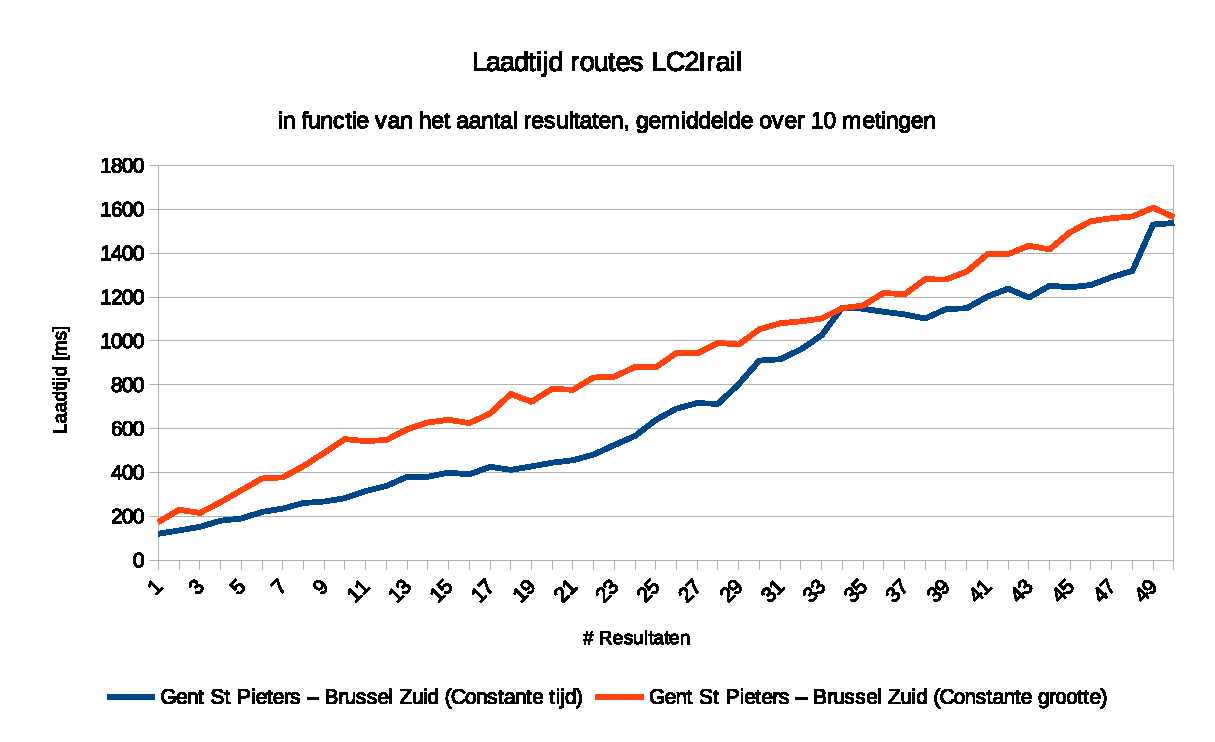
\includegraphics[width=1.00\textwidth]{images/Laadtijd_routes_Gent-St-Pieters_Brussel-Zuid.eps}
	
	\caption[Laadtijd routes tussen Gent en Brussel in functie van aantal resultaten]{De tijd die nodig is om routes te laden, met aankomst om 18u, in functie van het gewenste aantal resultaten.}
	\label{fig:responsetimeperresultsrouteBruSouth}
\end{figure} 

\begin{figure}[h]
	\centering
	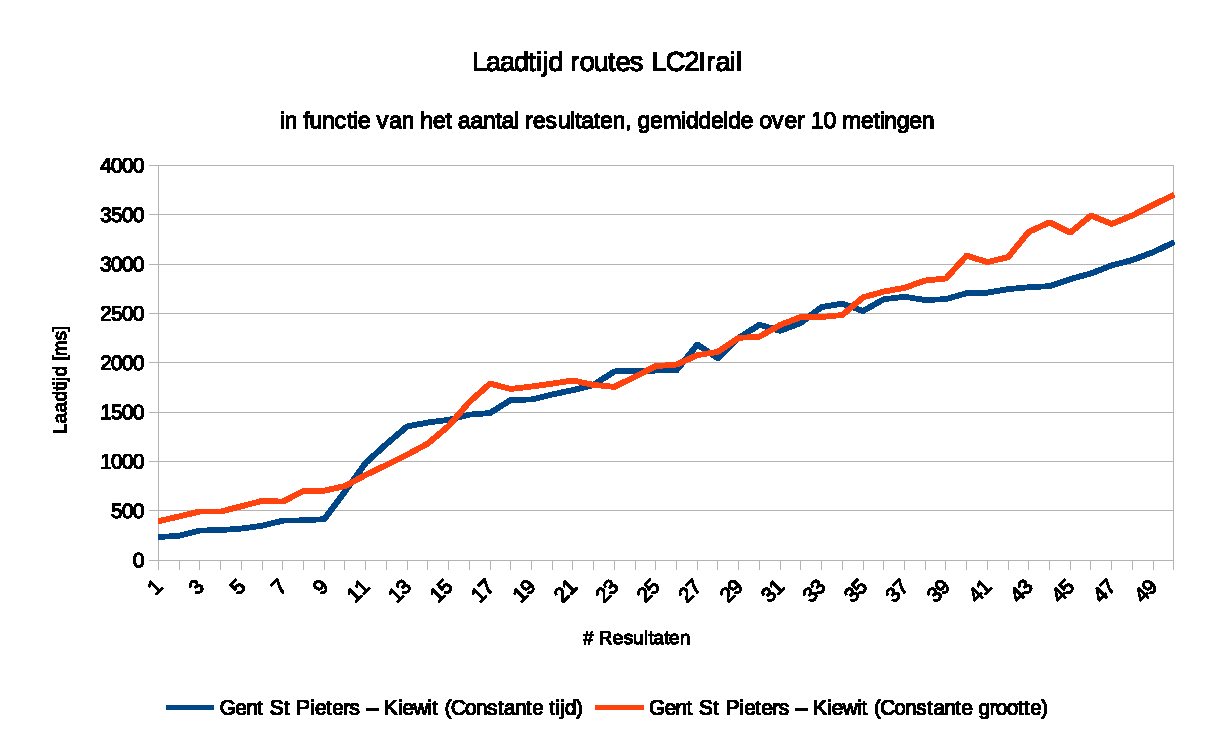
\includegraphics[width=1.00\textwidth]{images/Laadtijd_routes_Gent-St-Pieters_Kiewit.eps}	\caption[Laadtijd van routes tussen Gent en Kiewit in functie van aantal resultaten]{De tijd die nodig is om routes te laden, met aankomst om 18u, in functie van het gewenste aantal resultaten.}
	\label{fig:responsetimeperresultsrouteKiewit}
\end{figure}

We zien dat deze tijd telkens ongeveer lineair toeneemt, maar zeker de variant op basis van constante tijdsintervallen sterke knikken vertoont op sommige plaatsen. Deze knikken kunnen we verklaren aan het overlopen van pagina's met weinig connecties, zoals 's nachts wanneer geen treinen rijden en tijdens daluren. Sommige knikken die we in beide grafieken zien, worden veroorzaakt door pagina's met weinig relevante connecties. Dit is duidelijk merkbaar wanneer beide grafieken vergeleken worden: Tussen Gent en Brussel Zuid (een belangrijke treinverbinding) zijn er geen knikken wanneer gebruikgemaakt wordt van pagina's met een constante grootte, terwijl deze er wel zijn wanneer een route naar een klein station zoals Kiewit gepland wordt. Deze verschillen zijn zichtbaar in grafiek~\ref{fig:responsetimeperresultsroute}. Om te voorkomen dat gebruikers te lang moeten wachten op een resultaat wanneer een route naar een klein station gepland wordt, zal de server implementatie steeds 8 resultaten weergeven.

\begin{figure}[h]
	\centering
	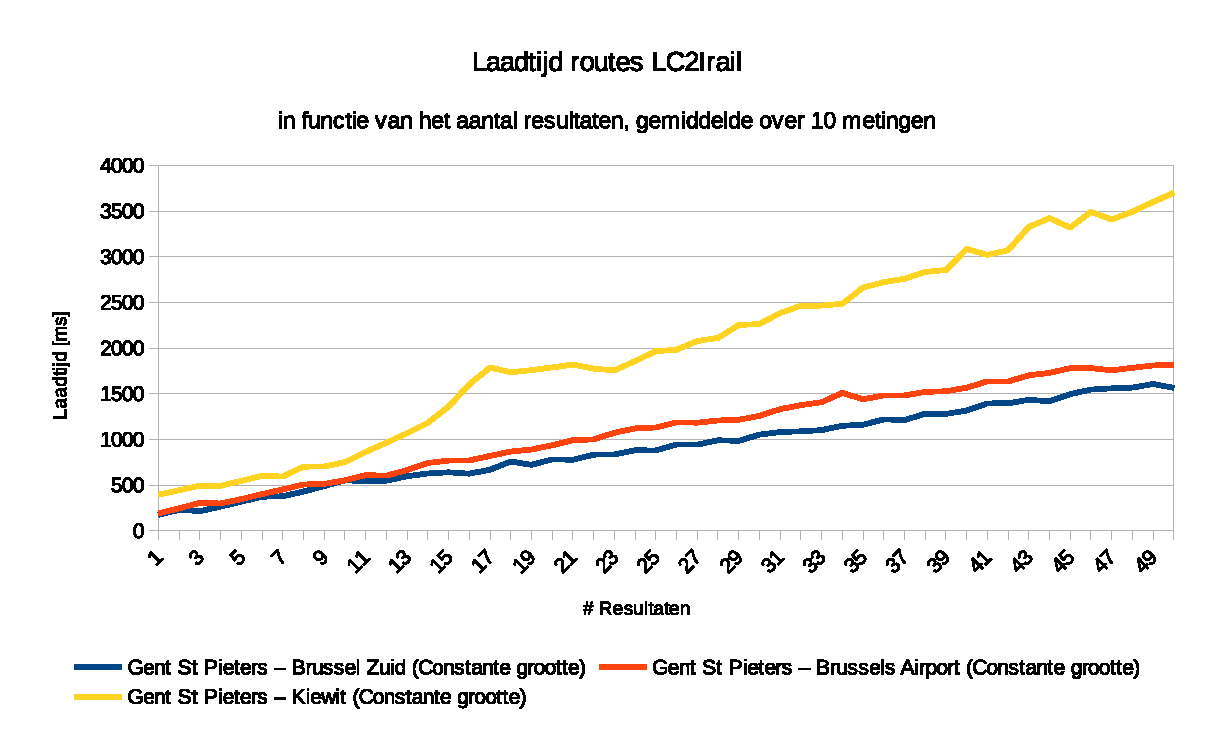
\includegraphics[width=1.00\textwidth]{images/Laadtijd_routes.eps}
	\caption[Laadtijd routes in functie van aantal resultaten]{De tijd die nodig is om routes te laden, met aankomst om 18u, in functie van het gewenste aantal resultaten. We zien een knik wanneer Linked Connections voor de nacht opgehaald worden, terwijl deze relatief weinig data bevatten.}
	\label{fig:responsetimeperresultsroute}
\end{figure}

Liveboards, die informatie geven over vertrekkende en aankomende treinen in een station, bouwen we op voor een bepaald interval. Gebruikers willen steeds informatie over treinen in de komende periode, en niet enkel de eerste resultaten, gezien ze niet op voorhand weten de hoeveelste trein ze zoeken. Ook voor liveboards onderzoeken we nu hoe lang het duurt om een deze op te bouwen voor een gegeven tijdsinterval. %TODO: zin nalezen.

\begin{figure}[h]
	\centering
	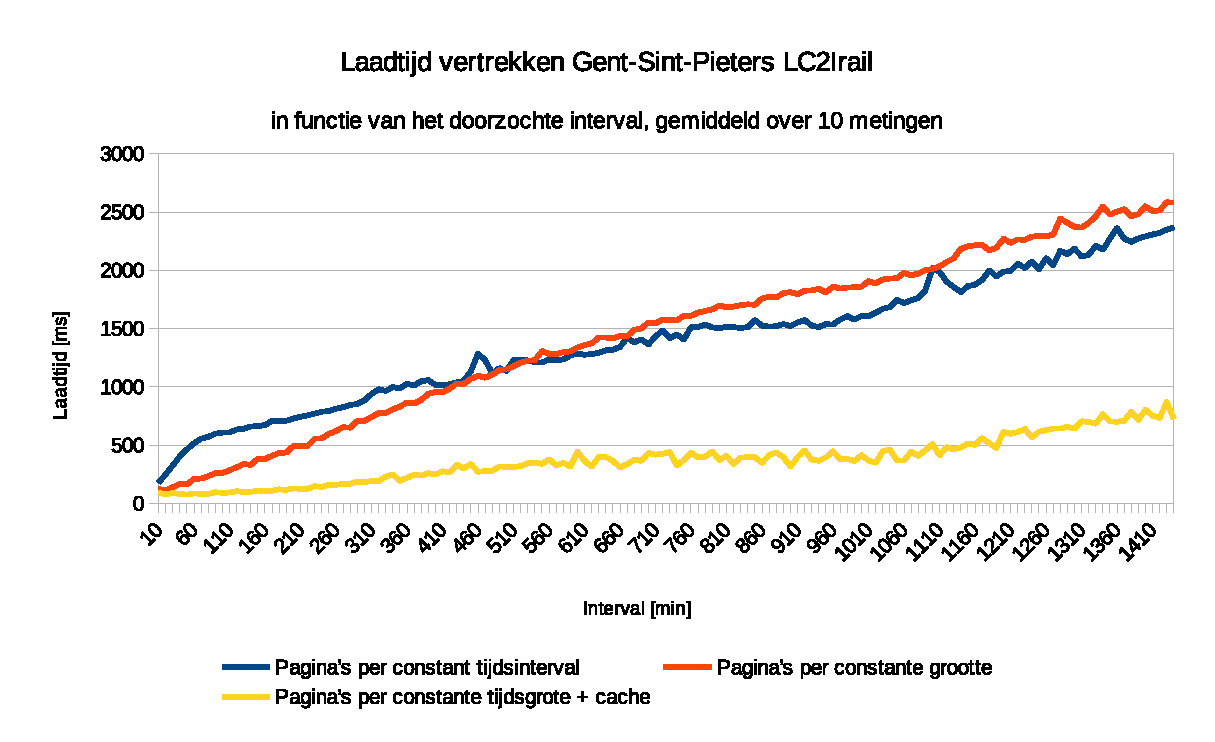
\includegraphics[width=1.0\textwidth]{images/Laadtijd_vertrekken.eps}
	\caption[Laadtijd liveboards in functie van het overlopen interval]{De tijd die nodig is om liveboards te laden over een bepaald interval.}
	\label{fig:responsetimeperintervalliveboards}
\end{figure}

\begin{figure}[h]
	\centering
	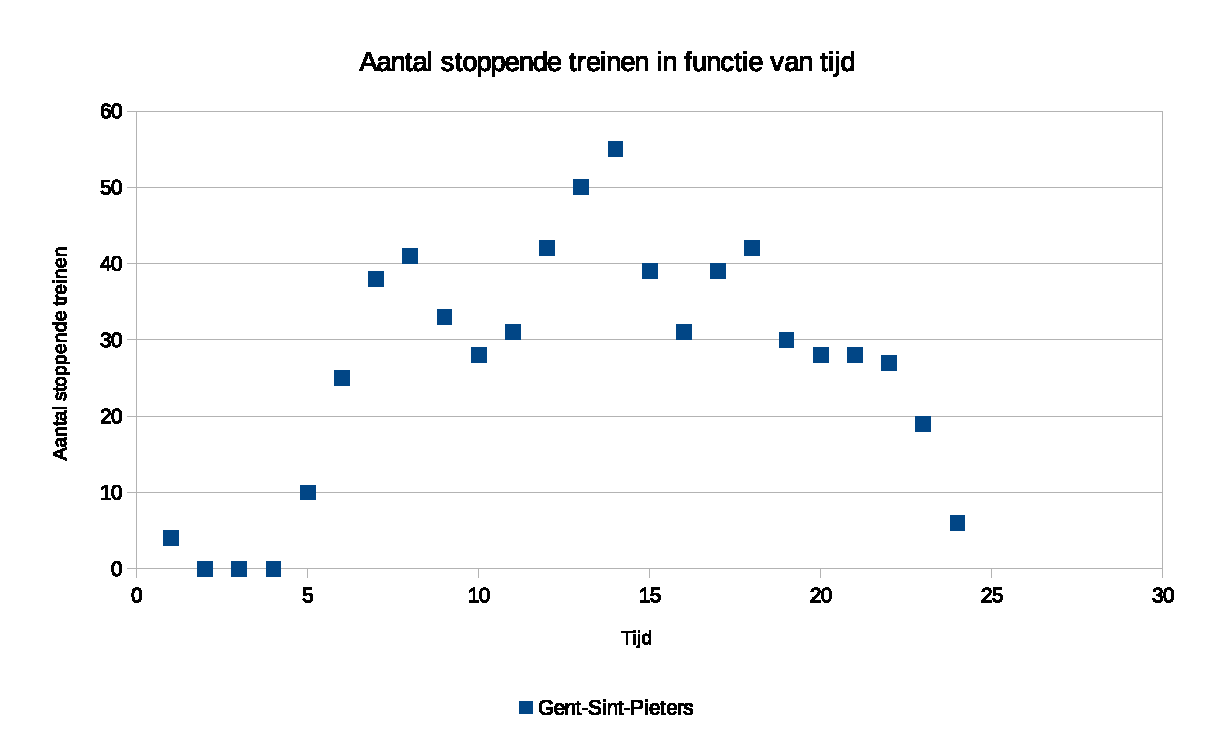
\includegraphics[width=1.0\textwidth]{StopsPerIntervalGhentStPietersBar.eps}
	\caption[Het aantal voertuigen die stoppen in Gent-St-Pieters]{Het aantal voertuigen die stoppen in Gent-Sint-Pieters op een werkdag.}
	\label{fig:stopsperintervaldetail}
\end{figure}

In grafiek~\ref{fig:responsetimeperintervalliveboards} zien we de tijd die benodigd is om een liveboard te genereren over een bepaald interval. In deze grafieken zien we dat bij pagina's van constante tijdintervallen de responstijd initieel sterk stijgt, waarna de curve een lineaire vorm aanneemt. Knikken in de curve kunnen we opnieuw wijten aan daluren, in dit geval zien we een vlak segment tussen 800 en 960 minuten. Dit komt ongeveer overeen met de periode tussen 1 en 4 uur 's nachts, waarin zeer weinig treinen rijden. Wanneer we in detail gaan kijken naar het aantal stops per interval van 30 minuten, zichtbaar in grafiek~\ref{fig:stopsperintervaldetail}, zien we duidelijk dat er een aantal uitschieters zijn rond de piekuren en 's middags, en momenten waarop er aanzienlijk minder treinen vertrekken, zoals in daluren en 's nachts. Deze fluctuaties zullen een effect hebben op zowel de server-side als client-side implementaties. Mogelijk zou dit ervoor kunnen zorgen dat de gebruikerservaring voor zoekopdrachten in de spits beter is dan voor zoekopdrachten 's nachts.

Wanneer we echter kijken naar de laadtijd bij pagina's van constante grootte, verloopt deze curve bijna lineair. De curve bevat geen vlakke segmenten meer, gezien alle pagina's aanwezig zijn. De toenemende laadtijd op momenten dat er geen treinen rijden is te wijten aan de implementatie: elke geladen pagina wordt volledig verwerkt. Bij gebruik van pagina's met een constante grootte zullen deze implementaties 's nachts dus resultaten geven die verder in de toekomst liggen, in plaats van geen resultaten. Wanneer gebruikgemaakt wordt van caching zien we dat de responstijd verder drastisch verlaagt. Het is deze variant die in productie gebruikt zal worden. 

Het is belangrijk om op te merken dat de metingen voor bovenstaande grafieken steeds gemaakt zijn op een lokale server, gebruik makend van krachtige hardware. Op zwakkere hardware zal de responstijd lineair hoger liggen. De LC2Irail applicatie wordt ingesteld om telkens 8 routes, en 60 minuten van vertrekken en aankomsten weer te geven. Hierdoor krijgt de gebruiker telkens genoeg resultaten, en wordt onnodig werk en tijdsverspilling vermeden.

\subsection{Caching}
Een van de grootste voordelen die bij Linked Connections hoort, is de hoge mate waarin data gecachet en hergebruikt kan worden. Om data te cachen zullen we een SQLite database bijhouden op de interne opslag van het toestel.

Door gebruik te maken van een opslag op het toestel blijven alle opgeslagen pagina's behouden wanneer de applicatie afgesloten en herstart wordt. Hierdoor is de applicatie ook na het afsluiten nog te gebruiken voor offline opzoekingen. Wanneer pagina's constante tijdsintervallen beschrijven is het eenvoudig om te controleren of een pagina reeds gecachet is: de gezochte tijd afronden, URL construeren en opzoeken in de database is voldoende. Wanneer echter pagina's van constante fysieke grootte gebruikt worden, kan het id van de pagina niet meer client-side bepaald worden. Wanneer een nog nooit eerder opgezocht tijdstip gezocht wordt, zoals 8:05, is het mogelijk dat deze data zich in de pagina beginnend op 8:03 bevindt. Om dit op te lossen gebruiken we een query, waarbij de URL voor een tijdstip geconstrueerd wordt en deze vergeleken wordt met de intervallen per pagina. De keuze voor SQLite laat toe om dit eenvoudig te implementeren. Een voorbeeld hiervan is te zien in fragment~\ref{code:2:LCCache}. In de cache slaan we steeds de URL, het volledige server antwoord en de tijd waarop het antwoord ontvangen werd op.

\begin{listing}[h]
	\begin{minted}[breaklines,tabsize=2]{java}
    db.query(TABLE, new String[]{"url", "data", "datetime"}, "url<=? AND next>?", new String[]{url,url}, null, null, "url DESC");
	\end{minted}
	\caption[Zoeken van pagina's in offline cache]{SQLite query om juiste pagina in cache te zoeken}
	\label{code:2:LCCache}
\end{listing}

Deze cache wordt gecontroleerd alvorens een verzoek te maken. Indien geen internet beschikbaar is, of de gecachete data minder dan 60 seconden oud is, wordt deze hergebruikt. Deze maximale ouderdom kan ook uit de HTTP-headers van de antwoorden onttrokken worden. De HTTP antwoord headers zijn echter niet onmiddellijk toegankelijk in de gebruikte bibliotheek, en om de ontwikkeltijd te verkorten, werd deze in het kader van deze masterproef echter hardgecodeerd.

\section{Optimalisatie verwerking op een mobiel toestel}
Bij de implementatie van Linked Connections in Android is vooral aandacht besteed aan de algoritmes. Efficiënte algoritmes zijn immers belangrijk voor het snel beantwoorden van de zoekopdracht door de gebruiker. Linked Connections parsen van JSON naar objecten wordt gedaan aan de hand van de standaard JSON parser in Android, org.json. Alle connecties van een pagina worden volledig geparset, alvorens de pagina verwerkt wordt door algoritmes. 
Tijdens user testing wordt het echter al snel duidelijk dat -- hoewel de app goed presteert op enkele testtoestellen en een emulator -- er ook verschillende gebruikers zijn bij wie de app enorm slecht presteert. Analyse van het CPU-gebruik door de applicatie\footnote{CPU verbruik kan niet exact gemeten worden, maar een indicatie van welke methodes het meest CPU tijd vereisen zijn wel mogelijk. Dit wordt verder besproken bij de beperkingen van dit onderzoek, sectie~\ref{sec:beperkingen}} duidt al snel aan dat er veel tijd besteed wordt aan het parsen van JSON, en ook specifiek aan het parsen van datums. Hierdoor duren opzoekingen, zowel online als offline, langer dan nodig. Het effect van de trage JSON parser wordt uitvergroot op tragere toestellen, waarbij het opzoeken van voertuigen enkele seconden langer kan duren vergeleken met een sneller toestel, ook als beide toestellen alle gegevens reeds in cache hebben.
Als oplossing wordt in eerste instantie het parsen van datums versneld: het tijdsformaat wordt expliciet gedefinieerd in een statische variabele, zodanig dat parsen hier optimaal verloopt. Ten tweede worden niet meer alle connecties volledig geparset: de ongeparsete JSON wordt opgeslagen in het LC-object, en velden worden slechts geladen wanneer nodig. Dit wil zeggen dat in het geval van liveboards enkel de vertrektijd en het vertrek- en eindstation van elke connectie geladen worden, in plaats van alle velden. Pas wanneer een connectie relevant wordt en andere velden nodig zijn, worden deze uit de JSON data geladen.
Deze aanpassingen zorgen voor een kleine verbetering, maar hebben geen al te grote impact: het laden van een voertuig gaat van gemiddeld 4500ms naar 3900ms op een HTC 10. Dit blijft enorm veel vanuit het standpunt van een gebruiker.
Wanneer we echter kijken naar een vergelijking tussen JSON parsers, blijkt al snel dat de standaard \foreign{org.json} parser bij de traagste parsers voor Java hoort\footnote{\url{https://github.com/fabienrenaud/java-json-benchmark}}. Dit is duidelijk te zien in figuur~\ref{fig:jsonparsersdeserialize}.

\begin{figure}[h]
	\centering
	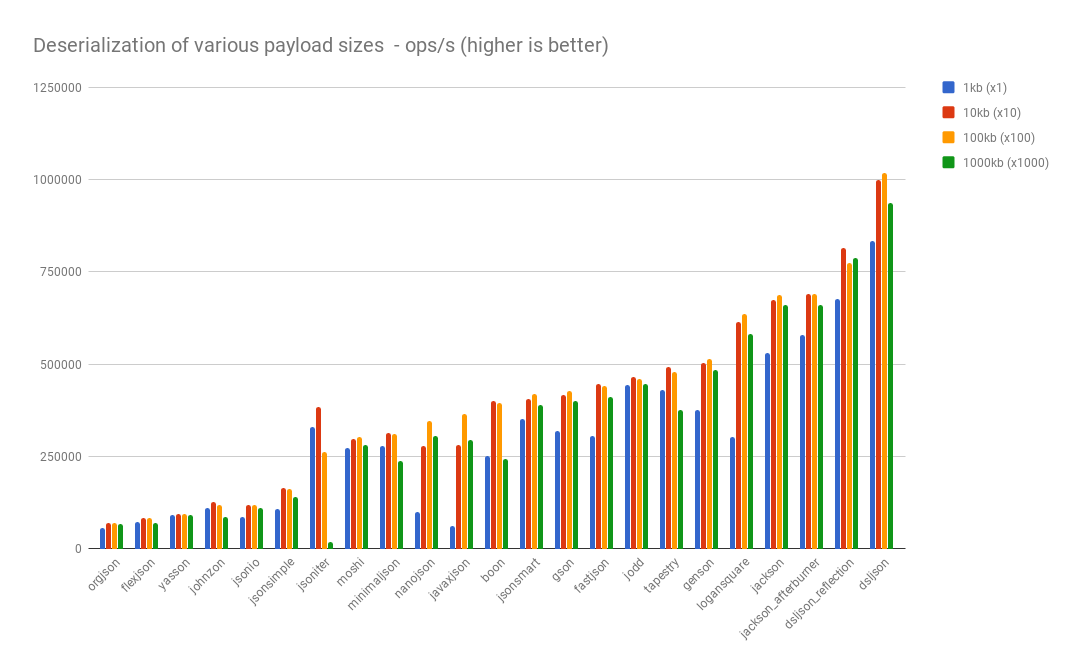
\includegraphics[width=1.0\textwidth]{jsondeserialization.png}
	\caption[Prestaties van JSON parsers]{Prestaties van verschillende JSON parsers bij deserialiseren. \textcopyright 2016 Fabien Renaud}
	\label{fig:jsonparsersdeserialize}
\end{figure}

Als oplossing is gekozen om de \foreign{LoganSquare} parser te gebruiken. \foreign{LoganSquare} is niet de snelste, maar wel aanzienlijk sneller dan \foreign{org.json} en relatief eenvoudig te implementeren. Deze parser is gebaseerd op Jackson, waardoor het grootste voordeel van Jackson gedeeld wordt: achterliggend wordt gebruikgemaakt van streaming, waardoor minder \foreign{garbage} veroorzaakt wordt. Hierdoor is minder \foreign{garbage collection} nodig, waardoor de code minder vaak gepauzeerd hoeft te worden en dus sneller resultaten geeft. De verschillen in performantie tussen de parsers worden besproken in hoofdstuk 4. Binnen de beperkte tijd die beschikbaar was voor het schrijven van deze masterproef was er onvoldoende tijd om \foreign{DSLJson} te implementeren. Afgaand op figuur~\ref{fig:jsonparsersdeserialize} zou hier echter wel nog prestatiewinst geboekt kunnen worden.